\documentclass[bwprint,a4paper]{extarticle}
\setcounter{tocdepth}{2}

\title{第一冊}
\author{666}
\date{}
\usepackage{amsmath,amssymb,gensymb,bm,fancyhdr,braket,mathrsfs}
\usepackage{multirow,multicol,ifthen,array,harpoon}
\usepackage{systeme,fancybox,times}
\usepackage{indentfirst,verbatim,subfigure,slashbox}  
\usepackage{url,booktabs,setspace,eso-pic,cellspace,scalerel}
\usepackage{makecell}
\usepackage{setspace}   % Set space between lines.
\usepackage{xspace}     % Define commands that appear not to eat spaces.
\usepackage{fontspec} %加這個就可以設定字體
\usepackage{xeCJK} %讓中英文字體分開設置
\setCJKmainfont{NotoSansTC-Regular.ttf}
\XeTeXlinebreaklocale "zh" 
\XeTeXlinebreakskip = 0pt plus 1pt
\usepackage{enumerate} %選擇題
\usepackage{amsfonts,amsthm,textcomp,tabularx,accents,extpfeil}
\usepackage{color} 
\usepackage{hyperref,afterpage}
\usepackage{framed}
\usepackage{enumitem}
\usepackage{varwidth}
\usepackage{hhline}%繪製特殊表格線
\usepackage{colortbl}%製作彩色表格
\usepackage{xcolor}%定義表格顏色
\usepackage{empheq}
\usepackage{graphicx}
	\definecolor{hellmagenta}{rgb}{1,0.75,0.9}
	\definecolor{hellcyan}{rgb}{0.75,1,0.9}
	\definecolor{hellgelb}{rgb}{1,1,0.8}
	\definecolor{colKeys}{rgb}{0,0,1}
	\definecolor{colIdentifier}{rgb}{0,0,0}
	\definecolor{colComments}{rgb}{1,0,0}
	\definecolor{colString}{rgb}{0,0.5,0}
	\definecolor{darkyellow}{rgb}{1,0.9,0}
	\definecolor{myblue}{RGB}{80,80,160}
	\definecolor{mygreen}{RGB}{80,160,80}
	\definecolor{shadecolor}{rgb}{0.87,0.87,0.87} 
	\def\xstrut{\vphantom{\dfrac{(A)^1}{(B)^1}}}
%\graphicspath{C:/Users/s0961/Desktop/自編講義}
\usepackage{qrcode}

% for drawing graphs
%\usepackage{tkz-fct,tikz-cd,pst-solides3d}
\usepackage{tikz,tkz-euclide,pst-eucl,pgf,pgfplots}
\usetikzlibrary{shapes,shapes.geometric}
\usetikzlibrary{decorations.markings,decorations.pathmorphing}
\usetikzlibrary{positioning,chains,fit,calc,intersections,tikzmark,through}
\usetikzlibrary{arrows,arrows.meta,automata,datavisualization,datavisualization.formats.functions}
\usetikzlibrary{graphs,graphs.standard,3d,perspective}

\tikzset{every picture/.style={thick}}
\tikzset{arrowMe/.style={postaction=decorate,decoration={markings, mark=at position .5 with {\arrow[thick]{#1}}}}}



\usepgfplotslibrary{polar}
\usepgflibrary{shapes.geometric}
\usepackage{forest}
\forestset{
  my tree/.style={
    before typesetting nodes={
      for tree={
        if={>O+tt=!O_=&{content}{}{n}{1}}{
          label/.process={Ow}{content}{left:##1},
        }{
          label/.process={Ow}{content}{right:##1},
       },
        content=,
      },
    },
    where level=0{
      draw,
      baseline,
      circle,
    }
    {
      draw,
      fill,
      circle,
    },
    for tree={inner sep=1.5pt, s sep'+=10pt},
  },
  default preamble={my tree},
  cut/.style={
    tikz+={
      \path [decorate, decoration={markings, mark=at position .5 with {\draw [] +(90:2.5pt) -- +(-90:2.5pt);}}] ()  -- (!u);
    }
  }
}
\thispagestyle{empty}
\pgfplotsset{my style/.append style={axis x line=middle, axis y line=
middle, xlabel={$x$}, ylabel={$y$}, axis equal }}

\newcommand{\mybox}[4][\textwidth-\pgfkeysvalueof{/pgf/inner xsep}-2mm]{%
\begin{figure}[!h]
\centering
\begin{tikzpicture}
\node[line width=.5mm, rounded corners, draw=#2, inner ysep=10pt, text width=#1, outer sep=0] (one) {\vspace*{15pt}\\\begin{varwidth}{\textwidth}#4\end{varwidth}};
\node[text=white,anchor=north east,align=center, minimum height=20pt] (two) at (one.north east) {#3 \hspace*{.5mm}};
\path[fill=#2]
    (one.north west|-two.west) --
    ($(two.west)+(-1.5cm,0)$)
    to[out=0,in=180] (two.south west) --
    (two.south east) [rounded corners] --
    (one.north east) --
    (one.north west) [sharp corners] -- cycle;
\node[text=white,anchor=north east,align=center, minimum height=20pt, text height=2ex] (three) at (one.north east) {#3 \hspace*{.5mm}};
\end{tikzpicture}
\end{figure}
}

\usepackage[most]{tcolorbox}
% user defined color
\usepackage{xcolor}
\definecolor{observecolor}{RGB}{153,201,227}
\definecolor{explorecolor}{RGB}{178,217,200}

\tcbset{
    common/.style={
		enhanced,
		arc=0mm,
		fonttitle=\large\bfseries,
		coltitle=black,
		attach boxed title to top left={xshift=0mm,
										yshift=-0.50mm},
		boxed title style={
			skin=enhancedfirst jigsaw,
			size=small,
			arc=5mm,
			bottom=0mm,
			left=8mm,
			right=18mm,
			top=1mm},
			boxrule=0pt,
			frame hidden},
	observestyle/.style={
		common,
		colbacktitle=observecolor,
		colframe=observecolor,
		colback=observecolor!40,
		borderline north={4pt}{0pt}{observecolor}}
}

\newtcolorbox{observe}{observestyle,title=小試身手}
\newtcolorbox{custom}[2][gray]{
	common,
	title=#2,
	colbacktitle=#1,
	colframe=#1,
	colback=#1!40,
	borderline north={4pt}{0pt}{#1}}


\usepackage[most]{tcolorbox}
% user defined color
\usepackage{xcolor}
\definecolor{observecolor}{RGB}{153,201,227}
\definecolor{explorecolor}{RGB}{178,217,200}

\tcbset{
    common/.style={
		enhanced,
		arc=0mm,
		fonttitle=\large\bfseries,
		coltitle=black,
		attach boxed title to top left={xshift=0mm,
										yshift=-0.50mm},
		boxed title style={
			skin=enhancedfirst jigsaw,
			size=small,
			arc=5mm,
			bottom=0mm,
			left=8mm,
			right=18mm,
			top=1mm},
			boxrule=0pt,
			frame hidden},
	observestyle/.style={
		common,
		colbacktitle=observecolor,
		colframe=observecolor,
		colback=observecolor!40,
		borderline north={4pt}{0pt}{observecolor}}
}

\newtcolorbox{observing}{observestyle,title=小試身手}
\newtcolorbox{customs}[2][brown]{
	common,
	title=#2,
	colbacktitle=#1,
	colframe=#1,
	colback=#1!40,
	borderline north={4pt}{0pt}{#1}}
\tcbuselibrary{skins,breakable,theorems}	

\makeatletter\long\def\ifnodedefined#1#2{\@ifundefined{pgf@sh@ns@#1}{}{#2}}\makeatother
\tikzset{
    %line-styles
        OO/.style={fill=blue,draw=blue,{Circle[width=1mm,length=1mm]}-{Circle[width=1mm,length=1mm]},shorten <= -0.5mm,shorten >= -0.5mm}, <O/.style={stealth-{Circle[width=1mm,length=1mm]},shorten <= 0mm}, O>/.style={{Circle[width=1mm,length=1mm]}-stealth,shorten >= 0mm}, <OO>/.style={stealth-stealth,shorten <= 0mm,shorten >= 0mm},every edge/.append style={OO},
    %how to plot:
        pics/.cd, plot inequality/.code n args={4}{
        %all the paths we need to figure out the intersections etc.
            \path[name path=conditionline] plot[variable=\x,domain={#2*1.01}:{#3*1.01},samples=300] ({\x},{ifthenelse(#1,{1+#4},{-1+#4})}); \path[name path=zeroline] (#2,#4) -- (#3,#4);\path[name path=start] (#2,{#4+1.1}) -- (#2,{#4+.9});\path[name path=end] (#3,{#4+1.1}) -- (#3,{#4+0.9});\path[name intersections={of=conditionline and start,name=startt}];\path[name intersections={of=conditionline and end,name=endd}];\path[name intersections={of=conditionline and zeroline,name=zerolinee}];\coordinate (intersection-0) at (#2,#4);
        %draw lines, nots and arrows
            \ifnum0\ifnodedefined{zerolinee-1}{1}\ifnodedefined{startt-1}{1}>0\draw[name intersections={of=zeroline and conditionline,total=\t,by=x}]\foreach \i [count=\s, evaluate=\s as \startswitch using iseven(\s+0\ifnodedefined{startt-1}{1})] in {0,...,{\t}}{\ifnum\i=\t coordinate (intersection-\s) at (#3,#4)\fi\if1\startswitch(intersection-\i) edge [\ifnodedefined{startt-1}{\ifnum\i=0<O\fi}\ifnodedefined{endd-1}{\ifnum\i=\t O>\fi}] (intersection-\s)\fi};\pgfnoderename{}{startt-1}\pgfnoderename{}{endd-1}\pgfnoderename{}{zerolinee-1}\fi}
}


% for margins
\usepackage[top=2.5cm,bottom=2.5cm,left=2cm,right=2cm,a4paper]{geometry}


% 表格高度及長內容換行
\newcommand{\xrowht}[2][0]{\addstackgap[.5\dimexpr#2\relax]{\vphantom{#1}}}
\newcommand{\tabincell}[2]{\begin{tabular}{@{}#1@{}}#2\end{tabular}}

%\setlength{\parindent}{2em}
% MACROS
\newenvironment{sol}{\medskip\noindent {\bf Solution.}}{\newpage}
\newcommand{\mystrut}{\rule[-.5\baselineskip]{0pt}{2\baselineskip}}
\newcommand{\divisible}{\mathrel{|}}
\newcommand{\bx}{{\bf x}}
\newcommand{\trans}{^\top}
\newcommand{\id}[1]{\ensuremath{\,\mathrm{d} #1}\xspace}
\newcommand{\eva}[1]{\ensuremath{\left.#1\right|}\xspace}
\newcommand{\ppair}[1]{\ensuremath{\left(#1\right)}\xspace}
\newcommand{\apair}[1]{\ensuremath{\left\langle#1\right\rangle}\xspace}
\newcommand{\bpair}[1]{\ensuremath{\left[#1\right]}\xspace}
\newcommand{\cpair}[1]{\ensuremath{\left\lceil #1\right\rceil}\xspace}
\newcommand{\fpair}[1]{\ensuremath{\left\lfloor #1\right\rfloor}\xspace}
\newcommand{\Bpair}[1]{\ensuremath{\left\{#1\right\}}\xspace} 
\newcommand{\vpair}[1]{\ensuremath{\left|#1\right|}\xspace}
\newcommand{\bmat}[1]{\ensuremath{\begin{bmatrix}#1\end{bmatrix}}\xspace} 
\newcommand{\Bmat}[1]{\ensuremath{\begin{Bmatrix}#1\end{Bmatrix}}\xspace} 
\newcommand{\vmat}[1]{\ensuremath{\begin{vmatrix}#1\end{vmatrix}}\xspace}
\newcommand{\Vmat}[1]{\ensuremath{\begin{Vmatrix}#1\end{Vmatrix}}\xspace} 
\newcommand{\pmat}[1]{\ensuremath{\begin{pmatrix}#1\end{pmatrix}}\xspace}
\renewcommand{\multirowsetup}{\centering} %合併表格後, 內容水平且垂直置中
%\renewcommand\arraystretch{1.8}%調整表格內行高
\newlength{\iconwidth} %定义ico标识的宽度
\setlength{\iconwidth}{1cm} %宽度赋值
\definecolor{boxheadcol}{gray}{.9} %定义所需的颜色,需要xcolor支持。
\definecolor{boxcol}{gray}{.5} %同上
\setlength\cellspacetoplimit{3pt}
\setlength\cellspacebottomlimit{3pt}
\setcellgapes{3pt}

%選擇題
\newcommand{\fourch}[4]{%~\hfill(\qquad)\\
\begin{tabular}{*{4}{@{}p{0.25\textwidth}}}(A)~#1 & (B)~#2 & (C)~#3 & (D)~#4\end{tabular}}
\newcommand{\twoch}[4]{%~\hfill(\qquad)\\
\begin{tabular}{*{2}{@{}p{0.5\textwidth}}}(A)~#1 & (B)~#2\end{tabular}\\\begin{tabular}{*{2}{@{}p{0.5\textwidth}}}(C)~#3 & (D)~#4\end{tabular}}
\newcommand{\onech}[4]{%~\hfill(\qquad)\\
(A)~#1 \\ (B)~#2 \\ (C)~#3 \\ (D)~#4}
\newlength\widthcha
\newlength\widthchb
\newlength\widthchc
\newlength\widthchd
\newlength\widthch
\newlength\tabmaxwidth
\setlength\tabmaxwidth{1\textwidth}
\newlength\fourthtabwidth
\setlength\fourthtabwidth{0.25\textwidth}
\newlength\halftabwidth
\setlength\halftabwidth{0.5\textwidth}

\newcommand{\choice}[4]{\settowidth\widthcha{AM.#1}\setlength{\widthch}{\widthcha}
    \settowidth\widthchb{BM.#2}
    \ifthenelse{\widthch<\widthchb}{\setlength{\widthch}{\widthchb}}{}
    \settowidth\widthchb{CM.#3}
    \ifthenelse{\widthch<\widthchb}{\setlength{\widthch}{\widthchb}}{}
    \settowidth\widthchb{DM.#4}
    \ifthenelse{\widthch<\widthchb}{\setlength{\widthch}{\widthchb}}{}
    \ifthenelse{\widthch<\fourthtabwidth}{\fourch{#1}{#2}{#3}{#4}}
    {\ifthenelse{\widthch<\halftabwidth\and\widthch>\fourthtabwidth}{\twoch{#1}{#2}{#3}{#4}}
        {\onech{#1}{#2}{#3}{#4}}}}

\everymath{\displaystyle} %所有數學模式都用展式數學模式
%填充題
%有計數的填充
%\newcounter{blanknumbering} % running number for filling blank 
%\def\blank{\addtocounter{blanknumbering}{1}
%\ensuremath{\underline{\hspace*{.5cm}\textcircled{\theblanknumbering}\hspace*{.5cm}}}}

%填充題
\def\blank{\ensuremath{\underline{\hspace*{1cm}}}}

%短除法
\newcounter{divline}
\def\rlwd{.5pt} \def\rlht{\dimexpr\dp\strutbox+\ht\strutbox} \def\rldp{.75ex}
\newcommand\mydiv[3][\relax]{%
  \ifx\relax#1\stepcounter{divline}\else\setcounter{divline}{#1}\fi%
  \mbox{}\hspace{\thedivline\dimexpr1ex}#2~\setbox0=\hbox{~$#3$}%
  \dumbstackengine{-\rlwd}{\rule[-\rldp]{\rlwd}{\rlht}~#3}{\rule{\dimexpr4pt+\wd0}{\rlwd}}%
}
\def\remainder#1{\stepcounter{divline}%
  \mbox{}\hspace{\dimexpr1ex+\thedivline\dimexpr1ex}~#1\setcounter{divline}{0}}
\makeatletter
\global\newlength\@stackedboxwidth
\newlength\@boxshift
\newsavebox\@addedbox
\newsavebox\@anchorbox
\newcommand*\dumbstackengine[3]{%
    \sbox{\@anchorbox}{$#2$}%
    \sbox{\@addedbox}{$#3$}%
    \setlength{\@stackedboxwidth}{\wd\@anchorbox}%
      \ifdim\wd\@addedbox>\@stackedboxwidth%
        \setlength{\@stackedboxwidth}{\wd\@addedbox}%
      \fi%
        \setlength{\@boxshift}{\dimexpr-\dp\@anchorbox -\ht\@addedbox -#1}%
        \usebox{\@anchorbox}%
        \hspace{-\wd\@anchorbox}%
        \raisebox{\@boxshift}{\usebox{\@addedbox}}%
        \hspace{-\wd\@addedbox}%
        \hspace{\@stackedboxwidth}%
}

\newtcbtheorem{question}{範例}%
  {enhanced, breakable,
    colback = white, colframe = cyan, colbacktitle = cyan,
    attach boxed title to top left = {yshift = -2mm, xshift = 5mm},
    boxed title style = {sharp corners},
    fonttitle = \sffamily\bfseries, separator sign = {~}}{qst}

% 直線表示
%\def\shrinkage{-2.4mu}
%\def\vecsign#1{\rule[1.388\LMex]{\dimexpr#1-2.5pt}{.36\LMpt}%
%  \kern-6.0\LMpt\mathchar"017E}
%\def\dvecsign#1{\rule{0pt}{7\LMpt}\smash{\stackon[-1.989\LMpt]{%
%  \SavedStyle\mkern-\shrinkage\vecsign{#1}}%
%  {\rotatebox{180}{$\SavedStyle\mkern-\shrinkage\vecsign{#1}$}}}}
%\def\dvec#1{\ThisStyle{\setbox0=\hbox{$\SavedStyle#1$}%
%  \def\useanchorwidth{T}\stackon[-4.2\LMpt]{\SavedStyle#1}{\,\dvecsign{\wd0}}}}
%\stackMath

% 頁首、頁眉
\fancyhead{}
\fancyhead[RO]{\textsc{\rightmark~~~~\thepage}}
\fancyhead[LE]{\textsc{\leftmark~~~~\thepage}}
\fancyfoot{}
\fancyfoot[RO,RE]{逆風特訓班}
%\fancyfoot[LO,LE]{\includegraphics[scale=0.1]{nsysu_logo}}
\renewcommand{\headrulewidth}{0.4pt}
\renewcommand{\footrulewidth}{0.4pt}

\begin{document}

\maketitle
\renewcommand{\contentsname}{目錄}
\pagenumbering{roman}
\setcounter{page}{1}
\tableofcontents
\newpage

\pagenumbering{arabic}
\setcounter{page}{1}
\pagestyle{fancy}


\newpage

\begin{center}
	\section{數與式}
\end{center}
\subsection{數與數線}


\subsubsection{負數的意義}
\mybox[12cm]{red!70!black}{重點觀念整理 $1$:二元一次式}{
\begin{enumerate}
\item 列式:\\
	含有兩種文字符號(二元)且兩種符號次方皆為一次,稱為二元一次式。\\
	ex:
	$$5x+3y,\ 200+x+2y,\ \frac{10}{17}\ x+y-6\cdots$$
\item 算式值:\\
	一個含有 $x,\ y$ 的二元一次式的值,由 $x\ \text{與}\ y$ 分別所代表的數來決定。\\
	ex:\\[12pt]
    $\begin{aligned}\hspace{15mm}
    	x=8,\ y=2
    	&\Rightarrow 5x+3y\\
    	&=5\times 8+3\times 2\\
    	&=46
    \end{aligned}$
\item 化簡:
	\begin{itemize}
		\item 同類項合併:相同的文字符號就是同類項且可以合併。\\
			ex: $ 2x,\ 5x\ \text{是同類項,}$\ $ -1,\ 5\ \text{也是同類項,但}\ 4x,\ 7\\ \text{不是同類項。}$
		\item 去括號法則:
		\begin{enumerate}
			\item 括號前為\ $+$ 號,去括號性質不變。\\
			ex: $ 6+(2x-3y)=6+2x-3y$
			\item 括號前為\ $-$ 號,去括號性質改變。\\
			ex: $ 6-(2x-3y)=6-2x+3y$
		\end{enumerate}
	\end{itemize}
\end{enumerate}}

\begin{question}{基本計算}{example}
	\begin{enumerate}
		\item $\epsilon$
		\item $\frac32\ppair{5x+3y-5}-\frac14\ppair{6x-2y+6}$
	\end{enumerate}
\end{question}
\vspace{15ex}
\begin{observing}
	\begin{enumerate}
		\item $ -\ppair{5x+2y-4}-\ppair{2x-3y+1}$
		\item $ \frac13\ppair{2x-y+1}-\frac23\ppair{4x+2y+5}$
	\end{enumerate}
\end{observing}
%\begin{tcolorbox}[arc=1mm, outer arc=4mm,title = {Tips}]
%This is a \textbf{tcolorbox} with title.
%\tcblower
%Here, you see the lower part of the box.
%\end{tcolorbox}
\vspace{5ex}
\subsubsection{數線與絕對值}
\mybox[13cm]{red!70!black}{重點觀念整理 $2$:二元一次方程式}{
\begin{enumerate}
\item 列二元一次方程式:\\
	某人的撲滿中有 $10$ 元硬幣 $x$ 個, $50$ 元硬幣 $y$ 個,共 $870$ 元,
	則可列出二元一次方程式 $10x+50y=870$。\\
	如上式,一個等式中包含未知數 $x,\ y$ 且未知數次方皆是一次,稱為二元一次方程式。
\item 二元一次方程式的解:\\
	將 $x,\ y$ 所代表的數代入方程式中,如果等號兩邊值相等,則 $x\ \text{與}\ y$ 就是二元一次方程式的解。\\
	ex:\\[12pt]
	判斷 $x=1,\ y=5$ 和 $x=-2,\ y=0$ 是不是 $2x+y=-4$ 的解?\\[12pt]
	解:\\[12pt]
    $\begin{aligned}\hspace{5mm}
    	&x=1,\ y=5
    	\Rightarrow 2x+y=2\times 1+5=7\neq-4\\
    	&x=-2,\ y=0\Rightarrow 2x+y=2\times -2+0=-4=-4
    \end{aligned}$\\[12pt]
    所以 $x=1,\ y=5$ 不是解, $x=-2,\ y=0$ 是解。
\end{enumerate}}
\begin{question}{基本題型}{example}
	\begin{enumerate}
		\item 第一次段考數學滿分 $100$ 分,選擇題 $10$ 題,每題 $4$ 分,填充題 $x$ 格,每格 $3$ 分,計算題 $y$ 題,每題 $8$ 分,依題意列二元一次方程式。\\
		\item 下表 $x,\ y$ 都是 $y=-x+6$ 的解,求值並填入表格中。\\
	\begin{center}
	\setlength{\tabcolsep}{7mm}{
		\begin{tabular}{|c|c|c|c|c|}
			\hline
			$x$ & $-2$ & {} & {} & $2$\\
			\hline
			$y$ & {} & $-2$ & $3$ & {}\\
			\hline
		\end{tabular}}
	\end{center}							 
	\end{enumerate}
\end{question}
\vspace{15ex}
\begin{observing}
	\begin{enumerate}
		\item 小名有 $x$ 元,姊姊有 $y$ 元,妹妹有 $100$ 元,小名與姊姊將身上所有錢的 $\cfrac25$ 給妹妹,則妹妹身上有多少錢?\\
		\item 下列哪些 $x,\ y$ 是方程式 $2x-5y=12$ 的解?\\[12pt]
		\choice{$x=1,\ y=2$}{$x=6,\ y=0$}{$x=-4,\ y=-4$}{$x=-9,\ y=-6$}
	\end{enumerate}
\end{observing}
\vspace{15ex}
\subsection{式的運算}

\subsubsection{整數四則運算與應用問題}
\mybox[10cm]{red!70!black}{重點觀念整理 $3$:二元一次聯立方程式}{
\begin{enumerate}
\item 列二元一次聯立方程式:\\
	兩個二元一次方程式合併在一起的式子,稱為二元一次聯立方程式。
\item 二元一次聯立方程式的解:\\
	將 $x,\ y$ 所代表的數代入聯立方程式中,如果同時滿足這兩個方程式,則 $x\ \text{與}\ y$ 就是二元一次聯立方程式的解。\\
	ex:\\[12pt]
	判斷 $x=2,\ y=6$ 是否為二元一次聯立方程式 
	$$\begin{cases}
		x+y=8\\[8pt]
		y=3x
	\end{cases}$$ 的解?\\[12pt]
	解:\\
    將 $x=2,\ y=6$ 代入得 
    $\begin{cases}
    	2+6=8\\[8pt]
    	6=3\times 2
    \end{cases}$
    所以 $x=2,\ y=6$ 是解。
\end{enumerate}}
\begin{question}{列方程式及解的檢驗}{example}
	\begin{enumerate}
		\item 六年九班男生人數比女生人數的 $2$ 倍少 $13$ 人,已知全班共 $32$ 人,如果男生有 $x$ 人、女生有 $y$ 人,則:
		\begin{enumerate}
			\item 由男生人數比女生人數的 $2$ 倍少 $13$ 人,可列得二元一次方程式為 $\underline{\hbox to 20mm{}}$。
			\item 由全班共 $32$ 人,可列得二元一次方程式為 $\underline{\hbox to 20mm{}}$。
		\end{enumerate}
		\item $ x=3,\ y=2$ 是哪個二元一次聯立方程式的解?\\[12pt]
		\choice{$\begin{cases}
    	2x+3y=12\\[8pt]
    	2x-y=8
    \end{cases}$}
    	{$\begin{cases}
    	3x+2y=12\\[8pt]
    	x-2y=4
    \end{cases}$}
    	{$\begin{cases}
    	x+3y=9\\[8pt]
    	4x-y=10
    \end{cases}$}
    	{$\begin{cases}
    	-3x+2y=5\\[8pt]
    	2x=3y
    \end{cases}$}
	\end{enumerate}
\end{question}
\vspace{15ex}
\begin{observing}
	\begin{enumerate}
		\item Robert 和 Ted 共 $260$ 元,其中 Robert 的錢是 Ted 的 $5$ 倍少 $100$ 元,如果 Robert 有 $x$ 元、Ted 有 $y$ 元,則:
		\begin{enumerate}
			\item 由Robert 的錢是 Ted 的 $5$ 倍少 $100$ 元,可列得二元一次方程式為 $\underline{\hbox to 20mm{}}$。
			\item 由總共 $260$ 元,可列得二元一次方程式為 $\underline{\hbox to 20mm{}}$。
		\end{enumerate}
		\item 下列哪組 $x,\ y$ 是二元一次聯立方程式
		$\begin{cases}
			x+y=2\\[8pt]
			3x-2y=11
		\end{cases}$ 的解?\\[12pt]
	 	\twoch{$x=5,\ y=-3$}{$x=3,\ y=-1$}{$x=7,\ y=5$}{$x=0,\ y=2$}			
	\end{enumerate}
\end{observing}

\newpage

\begin{center}
	\section{指、對數}
\end{center}

\subsection{指數}
\mybox[10cm]{red!70!black}{重點觀念整理 $1$:平面位置的描述和直角坐標}{
\begin{enumerate}
	\item 平面位置的描述:\\
		在同一直線上的點,可以用數線上的坐標來表達。
	\item 直角坐標(Cartesian coordinate):
		\begin{itemize}
			\item 平面上兩條互相垂直的數線,其交點稱為原點,以 $O$ 表示。
			\item 水平數線叫做 $x$ 軸(橫軸),向右表正向。
			\item 鉛垂數線叫做 $y$ 軸(縱軸),向上表正向。
			\item 這兩條數線所在的平面稱為直角坐標平面,簡稱坐標平面。
		\end{itemize}
	\item 數對與坐標:
		\begin{itemize}
			\item 在 $x$ 軸上坐標為 $-2$ 的位置,畫一條與 $x$ 軸垂直的直線,在 $y$ 軸上坐標為 $3$ 的位置,畫一條與 $y$ 軸垂直的直線,此兩條直線的交點 $P$ 為數對 $\ppair{-2,3}$ 所表之位置。
			\item $P(a,b)$ 在坐標平面上表示 $P$ 點的位置,其中 $a$ 是 $x$ 坐標, $b$ 是 $y$ 坐標。
			\item 若 $P(a,b)$ 為坐標平面上一點,則:
				\begin{itemize}
					\item[i.] $P$ 到 $x$ 軸的距離為 $|b|$ 單位長。
					\item[ii.] $P$ 到 $y$ 軸的距離為 $|a|$ 單位長。
				\end{itemize}
			\item 兩軸上點的坐標:
				\begin{itemize}
					\item[i.] $x$ 軸上坐標必為 $(a,0)$ 形式。
					\item[ii.] $y$ 軸上坐標必為 $(0,b)$ 形式。
				\end{itemize}
		\end{itemize}	
\end{enumerate}}
\newpage
\begin{question}{坐標平面上描點}{example}
	在下面坐標平面上,標示下列各點:\\[12pt]
	$A(1,3),\ B(3,5),\ C(-3,-3),\ D(-1,5),\ E(4,-5)$\\[12pt]
	
\end{question}
\begin{observing}
	在下面坐標平面上,標示下列各點:\\[12pt]
	$A(1,3),\ B(3,4),\ C(-2,-3),\ D(-1,2.5),\ E(2,-1)$\\[12pt]
	
\end{observing}
\begin{question}{求點坐標與兩軸之距離}{example}
	若 $A(-3,5)$ 為平面上一點,求:
	\begin{enumerate}[label=(\arabic*)]
		\item 過 $A$ 點作 $x$ 軸的垂線交 $x$ 軸於 $P$ 點,則 $P$ 點為何? $A$ 點與 $x$ 軸距離為多少?
		\item 過 $A$ 點作 $y$ 軸的垂線交 $y$ 軸於 $Q$ 點,則 $Q$ 點為何? $A$ 點與 $y$ 軸距離為多少?
	\end{enumerate}
\end{question}
\vspace{15ex}
\begin{observing}
	若 $P(a,b)$ 為平面上一點,過 $P$ 點作 $x$ 軸的垂線交 $x$ 軸於 $A$ 點 $(-2,0)$,交 $y$ 軸於 $B$ 點 $(0,-4)$ ,求:
	\begin{enumerate}[label=(\arabic*)]
		\item $P$ 點為何? 
		\item $P$ 點與 $x$ 軸和 $y$ 軸距離為多少?
	\end{enumerate}
\end{observing}
\vspace{20ex}
\subsubsection{質數的意義}
\mybox[11cm]{red!70!black}{重點觀念整理 $2$:點的移動及象限}{
\begin{enumerate}
	\item 水平移動:\\
		點 $(x,y)$ 往右/左移動 $a$ 個單位,新坐標為 $(x+a,y),\ (x-a,y)$。
	\item 垂直移動:\\
		點 $(x,y)$ 往上/下移動 $a$ 個單位,新坐標為 $(x,y+a),\ (x,y-a)$。
	\item $x$ 軸和 $y$ 軸將坐標平面分成四個象限:
		\begin{itemize}
			\item 第一象限 $(+,+)$:$x,\ y$ 坐標皆為正。
			\item 第二象限 $(-,+)$:$x,\ y$ 坐標分別為負、正。
			\item 第三象限 $(-,-)$:$x,\ y$ 坐標皆為負。
			\item 第四象限 $(+,-)$:$x,\ y$ 坐標分別為正、負。
			\item $x,\ y$ 軸上的點不屬於任何象限。
		\end{itemize}	
\end{enumerate}}
\begin{question}{求坐標的平移及周長和面積}{example}
	\begin{enumerate}
		\item 坐標平面上,由 $A$ 點 $(1,0)$ 出發,沿 $x$ 軸向左 $5$ 單位至 $B$ 點,再由 $B$ 點沿 $y$ 軸向上 $4$ 單位至 $C$ 點,求 $B,\ C$ 二點坐標為何?
		\item 如下圖,正方形 $ABCD$ 中,已知 $B(1,-3),\ D(-4,2)$,則:
		\begin{enumerate}[label=(\arabic*)]
			\item $C$ 點坐標為何?
			\item 正方形 $ABCD$ 周長和面積為多少?
		\end{enumerate}
		\begin{tikzpicture}[scale=0.5]
  			\draw (-4, -3) rectangle (1, 2);
  			\path
    		(-4, -3) node[below left] {$A$}
    		(1, -3) node[below right] {$B(1, -3)$}
    		(1, 2) node[above right] {$C$}
    		(-4, 2) node[above left] {$D(-4, 2)$};
		\end{tikzpicture}
		\item 已知 $A(2,3),\ B(-2,-1),\ C(4,-1)$ 三點,求三角形 $ABC$ 周長和面積。
	\end{enumerate}
\end{question}
\vspace{40ex}
\begin{observing}
	\begin{enumerate}
		\item 如下圖,長方形 $ABCD$ 中,已知 $A(-4,-1),\ C(1,2)$,則:
		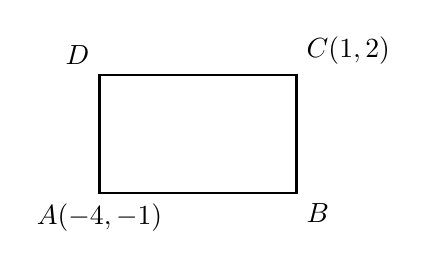
\begin{tikzpicture}[scale=0.5]
  			\draw (-4, -1) rectangle (1, 2);
  			\path
    		(-4, -1) node[below] {$A(-4,-1)$}
    		(1, -1) node[below right] {$B$}
    		(1, 2) node[above right] {$C(1,2)$}
    		(-4, 2) node[above left] {$D$};
		\end{tikzpicture}
		\begin{enumerate}[label=(\arabic*)]
			\item $D$ 點為何? 
			\item 長方形 $ABCD$ 周長和面積為多少?
		\end{enumerate}	
		\item 已知 $A(-1,5),\ B(-1,-3),\ C(-6,-1)$ 三點,求三角形 $ABC$ 周長和面積。	
	\end{enumerate}	
\end{observing}
\vspace{20ex}
\begin{question}{象限或軸上之判別}{example}
	\begin{enumerate}
		\item 判斷下列各點在哪一象限或哪一坐標軸上?\\
			  $A(3,4),\ B(-8,-7),\ C(6,-9),\ D(0,8),\ E(-3,0)$
		\item 若 $x>3,\ y<-2$,判斷下列各點在哪一象限內?
			\begin{enumerate}[label=(\arabic*)]
				\item $(x,y^2)$
				\item $(x-3,y+6)$
				\item $(xy,x-y)$
			\end{enumerate}
		\item 若 $P(x,y)$ 為平面上一點且 $ |x+3|+|2x-y+4|=0$,求:
			\begin{enumerate}[label=(\arabic*)]
				\item $x,\ y$ 之值
				\item $P$ 在第幾象限內?
			\end{enumerate}
	\end{enumerate}
\end{question}
\vspace{35ex}
\begin{observing}
	\begin{enumerate}
		\item 坐標平面上, $(ab,a)$ 在第三象限,判斷下列各點在哪一象限內?
			\begin{enumerate}[label=(\arabic*)]
				\item $(a^2,-b)$
				\item $(a-b,-a)$
				\item $(2b-3a,-b^2)$
			\end{enumerate}
		\item 若 $Q(x,y)$ 為平面上一點且 $\ppair{x-y+3}^2+\ppair{2x+y+5}^2=0$,求:
			\begin{enumerate}[label=(\arabic*)]
				\item $a,\ b$ 之值
				\item $Q$ 在第幾象限內?
			\end{enumerate}
	\end{enumerate}
\end{observing}
\vspace{30ex}
\subsubsection{質因數分解}
\mybox[13cm]{red!70!black}{重點觀念整理 $5$:二元一次聯立方程式的圖形}{
\begin{enumerate}
	\item 二元一次聯立方程式的圖形有以下 $3$ 種情況:\\[8pt]
\hspace{0.05\linewidth}
\begin{tabular}{|c|c|}
\hline
交於一點(恰有一組解) & 平行(無解)\\
\hline
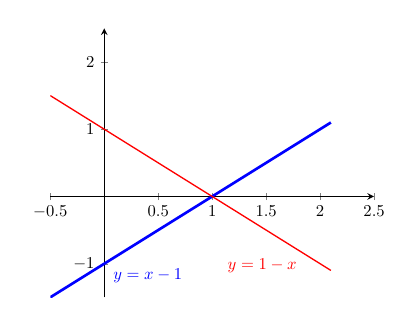
\begin{tikzpicture}[scale=0.6]
		\begin{axis}[
		axis lines = center,
		xmax = 2.5,
		ymax = 2.5,
%		ylabel = $y$,
%		xlabel = $x$,
		]
			\addplot[domain=-0.5:2.1,
					 smooth,
					 ultra thick,
					 blue,]{x-1}
					 node[pos=0.2, below right]{$y=x-1$};
			\addplot[domain=-0.5:2.1,
					 smooth,
					 thick,
					 red,]{1-x}
					 node[pos=0.9, below left]{$y=1-x$};
		\end{axis}	 
	\end{tikzpicture} &
	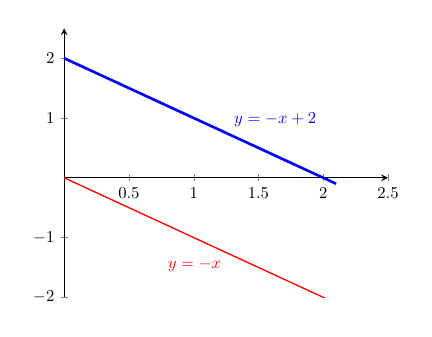
\begin{tikzpicture}[scale=0.6]
		\begin{axis}[
		axis lines = center,
		xmax = 2.5,
		ymax = 2.5,
		ymin = -2,
%		ylabel = $y$,
%		xlabel = $x$,
		]
			\addplot[domain=0:2.1,
					 smooth,
					 ultra thick,
					 blue,]{-x+2}
					 node[pos=0.6, above right]{$y=-x+2$};
			\addplot[domain=0:2.1,
					 smooth,
					 thick,
					 red,]{-x}
					 node[pos=0.6, below left]{$y=-x$};
		\end{axis}	 
	\end{tikzpicture}\\
\hline
\end{tabular}
\begin{center}
重合(無限多組解)\\[12pt]
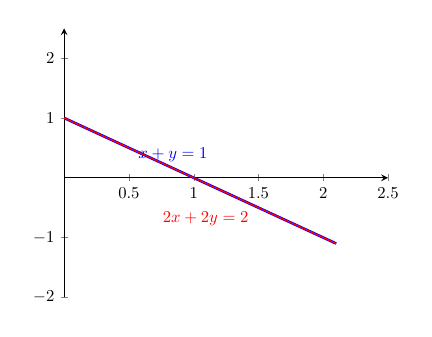
\begin{tikzpicture}[scale=0.6]
		\begin{axis}[
		axis lines = center,
		xmax = 2.5,
		ymax = 2.5,
		ymin = -2,
%		ylabel = $y$,
%		xlabel = $x$,
		]
			\addplot[domain=0:2.1,
					 smooth,
					 ultra thick,
					 blue,]{1-x}
					 node[pos=0.4, above]{$x+y=1$};
			\addplot[domain=0:2.1,
					 smooth,
					 thick,
					 red,]{1-x}
					 node[pos=0.7, below left]{$2x+2y=2$};
		\end{axis}	 
	\end{tikzpicture}
\end{center}
	\item 判斷二元一次聯立方程式解之情形:\\[8pt]
	$\begin{cases}
		a_1 x+b_1 y=c_1\\
		a_2 x+b_2 y=c_2
	\end{cases}
	,\ppair{a_1,\ a_2,\ b_1,\ b_2,\ c_1,\ c_2\neq0}$
		\begin{itemize}
			\item $\cfrac{a_1}{a_2}\neq\cfrac{b_1}{b_2}\Rightarrow
			\begin{cases}
				\text{恰有一解}\\
				\text{二直線相交於1點}\\
				\text{相容方程組}
			\end{cases}$
			\item $\cfrac{a_1}{a_2}=\cfrac{b_1}{b_2}\neq\cfrac{c_1}{c_2}\Rightarrow
			\begin{cases}
				\text{無解}\\
				\text{二直線平行}\\
				\text{矛盾方程組}
			\end{cases}$
			\item $\cfrac{a_1}{a_2}=\cfrac{b_1}{b_2}=\cfrac{c_1}{c_2}\Rightarrow
			\begin{cases}
				\text{$\infty$ 解}\\
				\text{二直線重合}\\
				\text{相依方程組}
			\end{cases}$
		\end{itemize}
\end{enumerate}
}
\begin{question}{畫聯立方程式之圖形及圖形判別}{example}
	\begin{enumerate}
		\item 畫出聯立方程式 
		$\begin{cases}
			x-y=3\\
			x+y=-1
		\end{cases}$ 的圖形並標出其交點坐標。
		\item 下列各聯立方程式之圖形,哪些是沒有交點?哪些是重合的直線?哪些是一個交點?\\[8pt]
		\twoch{$\begin{cases}
			2x-y=3\\
			2x+y=-1
		\end{cases}$}
		{$\begin{cases}
			3x-y=3\\
			3x+y=-1
		\end{cases}$}
		{$\begin{cases}
			-x-y=3\\
			-x+y=-1
		\end{cases}$}
		{$\begin{cases}
			2x-5y=5\\
			x+y=-1
		\end{cases}$}
	\end{enumerate}
\end{question}
\vspace{30ex}
\begin{observing}
	\begin{enumerate}
		\item 畫出聯立方程式 
		$\begin{cases}
			2x+y=4\\
			2x-y=0
		\end{cases}$ 的圖形並標出其交點坐標。
		\item 下列各聯立方程式之圖形,哪些是沒有交點?哪些是重合的直線?哪些是一個交點?\\[8pt]
		\twoch{$\begin{cases}
			4x-2y=-2\\
			-4x-y=-2
		\end{cases}$}
		{$\begin{cases}
			-x+3y=-2\\
			x-3y=2
		\end{cases}$}
		{$\begin{cases}
			5x+3y=1\\
			-5x-3y=1
		\end{cases}$}
		{$\begin{cases}
			2x-3y=4\\
			x+y=-2
		\end{cases}$}
	\end{enumerate}
\end{observing}
\newpage
\begin{customs}{功力UPUP}
	\begin{enumerate}
		\item 若 $A(5,8),\ B(3,2),\ C(k,k+1)$ 三點在同一線上,求 $k$ 及此方程式。
		\item 設 $a,\ b$ 為已知且 $a,\ b\neq0$,在坐標平面上,若直線 $ \frac{x}{a}+\frac{y}{b}=1$ 不通過第四象限,則 $(a,b)$ 在哪個象限?
		\item 已知某颱風行徑路線是直線,$(143,52),\ (145,58)$ 分別是早上6時和8時的颱風中心位置,求下午2時颱風中心位置?
		\item $A(7,11),\ B(–9,11),\ C(m, n)$ 為直角坐標平面上三點且 $\overline{AC}=\overline{BC},\ \overline{CD}\perp\overline{AB}$ 且 $\bigtriangleup ABC$ 的面積為 $104$,求 $C$ 點的坐標。
	\end{enumerate}
	%\qrcode[height=0.5in]{https://www.ctan.org/tex-archive/macros/latex/contrib/qrcode?lang=en}
\end{customs}


\subsection{常用對數}

\subsubsection{最大公因數}
\mybox[13cm]{red!70!black}{重點觀念整理 $3$:$ax+by=c$ 的圖形}{
\begin{enumerate}
	\item 二元一次方程式解的圖形:\\
		  一個二元一次方程式任意一組解,可以視為數對的形式,這一組解在平面上圖形就是一個點。\\
		  ex: \\[8pt]
		  $x=0,\ y=5$ 是二元一次方程式 $x+3y=15$ 的一組解,這組解的圖形就是坐標平面上 $(0,5)$ 這一點。
	\item 二元一次方程式的圖形:
		\begin{enumerate}[label=(\arabic*)]
			\item 一個二元一次方程式的所有解,畫在坐標平面上所形成的圖形,稱為該方程式的圖形。
			\item 快速畫出二元一次方程式的圖形:\\
				  找出二組解(通常取 $x,\ y=0$),在坐標平面上描出此二點,並畫出通過此二點的直線。
			\item 形如 $ax+by=c,\ (a,\ b\neq0)$ 之二元一次方程式,其圖形在平面上是一條線,該直線上所有點都代表方程式的一組解。
			\item 二元一次方程式 $ax+by=c$ 的圖形是一條直線,如果 $c=0$,則此直線會通過原點。
		\end{enumerate}
\end{enumerate}
\begin{minipage}{\linewidth}
\hspace{0.1\linewidth}
\begin{minipage}{0.3\textwidth}
	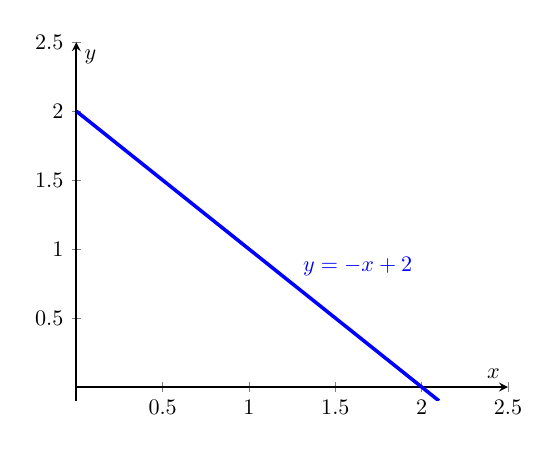
\begin{tikzpicture}[scale=0.8]
		\begin{axis}[
		axis lines = center,
		xmax = 2.5,
		ymax = 2.5,
		ylabel = $y$,
		xlabel = $x$,
		]
			\addplot[domain=0:2.1,
					 smooth,
					 ultra thick,
					 blue,]{-x+2}
					 node[pos=0.6, above right]{$y=-x+2$};
%			\addplot[domain=-2:3,
%					 smooth,
%					 thick,
%					 red,]{x};
%			\addplot[domain=-2:2,
%					 smooth,
%					 thick,
%					 black,]{x-1};
		\end{axis}	 
	\end{tikzpicture}
\end{minipage}
\hspace{0.2\linewidth}
\begin{minipage}{0.3\textwidth}
	\par\vspace{1pt}
	 以左圖來說,將 $(0,2),\ (1,1),\ (2,0),\cdots$	 代入,會是 $y=-x+2$ 的解且圖形是一條線。
\end{minipage}
\end{minipage}
}
\newpage

\begin{question}{畫出方程式及求通過直線上的點}{example}
	\begin{enumerate}
		\item 在坐標平面上畫出二元一次方程式 $2x+5y=4$ 的圖形。	  
		\item 已知 $(3,a),\ (b,-2)$ 都在 $5x-3y=15$ 上,求數對 $(a,b)=$?
		\item 在坐標平面上,若直線 $3x-(2k-1)y=6-2k$ 通過原點,求 $k$ 及直線方程式。
	\end{enumerate}
\end{question}
\vspace{40ex}
\begin{observing}
	\begin{enumerate}
		\item 在坐標平面上畫出二元一次方程式 $x-5y=10$ 的圖形。	  
		\item 已知 $P(2,3)$ 在 $2x+ay=7$ 上,求 $a=$?
		\item 在坐標平面上,若直線 $2x-y+2m-4=0$ 通過原點與 $(-3,n)$,求 $m,\ n$。
	\end{enumerate}
\end{observing}
\newpage
\subsubsection{最小公倍數}
\mybox[13cm]{red!70!black}{重點觀念整理 $4$:直線方程式圖形的類型}{
\hspace{0.08\linewidth}
\begin{tabular}{|c|c|}
\hline
圖一 & 圖二\\
\hline
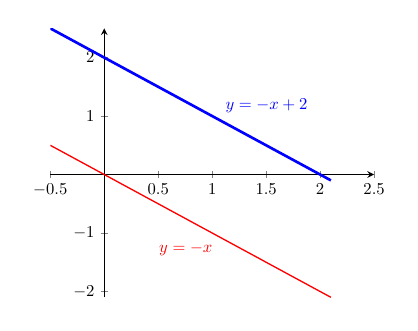
\begin{tikzpicture}[scale=0.6]
		\begin{axis}[
		axis lines = center,
		xmax = 2.5,
		ymax = 2.5,
%		ylabel = $y$,
%		xlabel = $x$,
		]
			\addplot[domain=-0.5:2.1,
					 smooth,
					 ultra thick,
					 blue,]{-x+2}
					 node[pos=0.6, above right]{$y=-x+2$};
			\addplot[domain=-0.5:2.1,
					 smooth,
					 thick,
					 red,]{-x}
					 node[pos=0.6, below left]{$y=-x$};
		\end{axis}	 
	\end{tikzpicture} &
	\begin{tikzpicture}[scale=0.6]
		\begin{axis}[
		axis lines = center,
		xmax = 2.5,
		ymax = 2.5,
		ymin = -2,
%		ylabel = $y$,
%		xlabel = $x$,
		]
			\addplot[domain=0:2.1,
					 smooth,
					 ultra thick,
					 blue,]{2}
					 node[pos=0.6, above right]{$y=2$};
			\addplot[domain=0:2.1,
					 smooth,
					 thick,
					 red,]{-1}
					 node[pos=0.6, below right]{$y=-1$};
		\end{axis}	 
	\end{tikzpicture}\\
\hline
\end{tabular}\\
\begin{center}
%	\includegraphics[scale=0.45]{vertical}\\
\end{center}
\centering 圖三
\begin{enumerate}
	\item 方程式 $ax+by=c,\ (a,\ b\neq0)$ 其圖形為一條斜直線,例如:$y=-x+2$。當 $c=0$,該直線會通過原點,例如:$y=-x$ (圖一)。
	\item 
		\begin{enumerate}[label=(\arabic*)]
			\item $y=k,\ k\neq0$,其圖形為通過 $y$ 軸上 $k$ 那點且與 $y$ 軸垂直的直線,例如:$y=-1$。
			\item $y=0$,其圖形為 $x$ 軸(圖二)。
		\end{enumerate}
	\item 
		\begin{enumerate}[label=(\arabic*)]
			\item $x=0$,其圖形為 $y$ 軸。
			\item $x=h,\ h\neq0$,其圖形為通過 $x$ 軸上 $h$ 那點且與 $x$ 軸垂直的直線,例如:$x=2$ (圖三)。
		\end{enumerate}
\end{enumerate}
}
\newpage
\begin{question}{求方程式與兩軸所圍之圖形}{example}
	\begin{enumerate}
		\item 求下列直線方程式:
		\begin{enumerate}[label=(\arabic*)]
			\item 通過 $(4,-5)$ 且平行 $x$ 軸的直線方程式。	  
			\item 通過 $(4,-5)$ 且平行 $y$ 軸的直線方程式。
		\end{enumerate}	
		\item 已知 $(3,1),\ (-4,-2)$ 都在 $ax+by=1$ 上,求數對 $(a,b)$ 及此直線方程式。
		\item 坐標平面上 $O$ 為原點且直線 $y=2x+6$ 分別交 $x,\ y$ 軸於 $A,\ B$ 二點,求 $A,\ B$ 及 $\bigtriangleup OAB$ 的面積。
	\end{enumerate}
\end{question}
\vspace{45ex}
\begin{observing}
	\begin{enumerate}
		\item 坐標平面上一直線 $y=ax+b$ 通過 $(1,8),\ (-2,5)$ 兩點,求此直線方程式。 
		\item 坐標平面上直線 $ax-3y=8$ 交 $x$ 軸於 $(2,0)$,求 $a$ 及與兩軸所圍之三角形的面積。
	\end{enumerate}
\end{observing}
\newpage

\begin{center}
	\section{多項式函數}
\end{center}

\subsection{多項式的運算與應用}

\subsubsection{一元一次式的意義、值與化簡}
\mybox[13cm]{red!70!black}{重點觀念整理 $1$:比與比值}{
\begin{enumerate}
	\item 兩個數 $a,\ b\ (b\neq0)$ 的比,記作 $a:b$,其中 $a$ 為前項,$b$ 為後項,其比值為 $a\div b\ppair{=\cfrac{a}{b}}$,表示 $a$ 是 $b$ 的 $\cfrac{a}{b}$ 倍。
	\item 比值相等的兩個比稱為相等的比。
	\item 比的擴分與約分:一個比的前項與後項同乘/除以一個不為零的數,其值仍不變。\\
		ex:\\[8pt]
		$\begin{aligned}
			&a:b=(a\times m):(b\times m),\ m\neq0\\
			&a:b=(a\div m):(b\div m),\ m\neq0
		\end{aligned}$	
	\item 一個比的前、後項為互質的兩整數,稱為最簡整數比。
\end{enumerate}
}
\begin{question}{基本題型}{example}
	\begin{enumerate}
		\item 甲甲國中全校 $1600$ 位學生,若戴眼鏡的同學有 $768$ 人,則未戴眼鏡的同學和有戴眼鏡的同學的筆是多少?其比值?
		\item 一個鐵塊重 $3\ kg$,一塊石頭重 $360\ g$,則重量比?其比值?
		\item 求出比值:
		\begin{enumerate}[label=(\arabic*)]
			\item $\cfrac52:\cfrac53$
			\item $3.2:3.4$
			\item $3\cfrac34:2\cfrac17$
		\end{enumerate}
		\item $A,\ B$ 兩個杯子各裝 $120\ ml,\ 200\ ml$ 的水,現在各滴入蜂蜜 $2,\ 3$ 滴,如果滴蜂蜜的量都相同,則哪一杯甜度比較高?
		\item 將下列各式化為最簡整數比:
		\begin{enumerate}[label=(\arabic*)]
			\item $\cfrac15:\cfrac17$
			\item $54:72$
			\item $1\cfrac34:2\cfrac17$
		\end{enumerate}
	\end{enumerate}
\end{question}
\vspace{30ex}
\begin{observing}
	\begin{enumerate}
		\item 求出比值:
		\begin{enumerate}[label=(\arabic*)]
			\item $\cfrac73:\cfrac53$
			\item $5.1:3.4$
			\item $6\cfrac35:3\cfrac14$
		\end{enumerate}
		\item 將下列各式化為最簡整數比:
		\begin{enumerate}[label=(\arabic*)]
			\item $2.8:4.2$
			\item $75:45$
			\item $2\cfrac34:7\cfrac13$
		\end{enumerate}
		\item 今年學測考試,甲校 $600$ 人報考,錄取 $150$ 人;乙校 $900$ 人報考,錄取 $210$ 人;丙校 $300$ 人報考,錄取 $60$ 人,則哪個學校錄取率最高?
	\end{enumerate}
\end{observing}
\newpage

\subsection{簡單多項式函數及其圖形}

\subsubsection{一元一次方程式的列式與解}
\mybox[11cm]{red!70!black}{重點觀念整理 $1$:正比}
{\hspace{0.5cm}$x,\ y$ 關係式中,當 $x$ 值改變時,$y$ 值也隨之改變且 $y:x$ 之比值為定值 $k$,稱作 $x,\ y$ 成正比,可以寫成 $y=kx,\ (k\neq0)$。
}
\begin{question}{正比的應用}{example}
	\begin{enumerate}
		\item 設 $y\ \text{與}\ x$ 成正比,當 $x=6,\ y=5$,則:
		\begin{enumerate}[label=(\arabic*)]
			\item $y\ \text{與}\ x$ 的關係式?
			\item 當 $x=\cfrac13,\ y=?$
		\end{enumerate}
		\item 已知寶石的價格與重量的平方成正比。有一塊寶石價值 $1000000$ 元,今不慎摔成兩塊,其重量比為 $2:3$,試問損失多少元。
		\item 設一彈簧在彈性限度內至多可秤重 $50\ kg$,已知秤重 $30\ kg$ 的物體時,彈簧被拉長 $6\ cm$,試問秤重 $40\ kg$ 的物體時,彈簧被拉長多少?
	\end{enumerate}	
\end{question}
\newpage
\begin{observing}
	\begin{enumerate}
		\item 設 $y\ \text{與}\ x$ 成正比,當 $x=\cfrac{14}3,\ y=\cfrac76$,則:
		\begin{enumerate}[label=(\arabic*)]
			\item $y\ \text{與}\ x$ 的關係式?
			\item 當 $y=250,\ x=?$
		\end{enumerate}
		\item 已知不考慮空氣與阻力的情況下,自由落體落下的距離隨時間的平方成正比。若某物體自高處落下,在 $2$ 秒內落下了 $19.6\ m$,試問:
		\begin{enumerate}[label=(\arabic*)]
			\item 該物體在 $4$ 秒內落下多少?
			\item 該物體在第 $4$ 秒內落下多少?
		\end{enumerate}
	\end{enumerate}	
\end{observing}
\vspace{45ex}
\subsubsection{解一元一次方程式}
\mybox[11cm]{red!70!black}{重點觀念整理 $2$:反比}
{\hspace{0.5cm}$x,\ y$ 關係式中,當 $x$ 值改變時,$y$ 值也隨之改變且 $y:x$ 之乘積為定值 $k$,稱作 $x,\ y$ 成反比,可以寫成 $xy=k,\ (k\neq0)$。
}
\newpage
\begin{question}{反比的應用}{example}
	\begin{enumerate}
		\item 設 $y\ \text{與}\ x$ 成反比,當 $x=\cfrac3{14},\ y=\cfrac76$,則:
		\begin{enumerate}[label=(\arabic*)]
			\item $y\ \text{與}\ x$ 的關係式?
			\item 當 $x=300,\ y=?$
		\end{enumerate}
		\item 若 $25000$ 元的存款每年可得利息 $1000$ 元,如果想獲得 $1600$ 元利息,那麼要增加多少元存款?
		\item 有一工程,已知 $10$ 個工人合作,$24$ 日可完工,今若要提早 $4$ 日完工,需增加多少工人?
	\end{enumerate}	
\end{question}
\vspace{30ex}
\begin{observing}
	\begin{enumerate}
		\item 設 $y\ \text{與}\ x$ 成反比,當 $x=3,\ y=-\cfrac16$,則:
		\begin{enumerate}[label=(\arabic*)]
			\item $y\ \text{與}\ x$ 的關係式?
			\item 當 $y=\cfrac25,\ x=?$
		\end{enumerate}
		\item 從 $A\ \text{到}\ B$ 地甲花了 $3\cfrac13$ 時到達,乙花了 $3\cfrac34$ 時到達,則甲乙之速度比?
		\item 有一件事,甲一人獨做 $8$ 天完成,乙一人獨做 $12$ 天完成,丙一人獨做 $16$ 天完成,則甲乙丙三人每天能力之比?
	\end{enumerate}	
\end{observing}
\newpage
\begin{customs}{功力UPUP}
	\begin{enumerate}
		\item 汽車從 $A\ \text{到}\ B$ 以每小時 $75\ km$ 速度行駛需 $2$ 小時到達,若回程速度增加 $20\%$,則來回共花多久?
		\item 若 $\frac{1}{2x+1}\ \text{與}\ \frac{1}{y-4}$ 成反比且當 $x=1\ \text{時},\ y=0$,則當 $y=8,\ x=?$
		\item 設 $y\ \text{與}\ x^2$ 成反比,當 $x$ 增加 $3$ 倍時,則 $y$ 變為原本多少倍?
		\item 甲乙丙同時出發跑 $400\ m$,若三人全程均以固定速率來跑,當乙到終點時,甲離終點還有 $50\ m$,丙離終點還有 $100\ m$ ,那麼:
		\begin{enumerate}[label=(\arabic*)]
			\item 甲、乙、丙三人速率比。
			\item 三人以相同速率參加 $800\ m$ 比賽,當丙落後乙 $70\ m$ 時,乙離終點還有多少?
		\end{enumerate}
	\end{enumerate}
	%\qrcode[height=0.5in]{https://www.ctan.org/tex-archive/macros/latex/contrib/qrcode?lang=en}
\end{customs}
\subsection{多項式函數的圖形與多項式不等式}

\subsubsection{一元一次方程式的應用問題}
\newpage
\begin{center}
	\section{直線與圓}
\end{center}

\subsection{直線方程式及其圖形}
\subsubsection{認識三角形、四邊形、多邊形(含點、線、角)}
\mybox[13cm]{red!70!black}{重點觀念整理 $1$:認識一元一次不等式}{
\begin{enumerate}
	\item 三一律:\\
		\hspace{0.5cm}任意兩數 $a,\ b$ 之間的大小關係有三種情形,即 $a>b,\ a=b,\ a<b$,其中恰好有一種會成立。
	\item 遞移律:
		\begin{enumerate}[label=(\arabic*)]
			\item $a>b,\ b>c\Rightarrow a>c$
			\item $a<b,\ b<c\Rightarrow a<c$
			\item $a=b,\ b=c\Rightarrow a=c$
		\end{enumerate}
	\item 不等式:\\
		\hspace{0.5cm}$<,\ >,\ \leq,\ \geq,\ \neq$ 都稱為不等號;含不等號的式子,稱為不等式。
	\item 常見不等號的讀法及其同義詞:\\[12pt]
		\begin{tabular}{|c|c|c|}
			\hline
			符號 & 讀法 & 同義詞舉例\\
			\hline
			$>$ & 大於 & 超過、高於\\
			\hline
			$<$ & 小於 & 不足、不滿、不到、低於\\
			\hline
			$\leq$ & 小於或等於 & 不大於、不高於、至多、以下(含)、不超過\\
			\hline
			$\geq$ & 大於或等於 & 不小於、不低於、至少、以上(含)\\
			\hline
			$\neq$ & 不等於 & 不相等、相異、非\\
			\hline
		\end{tabular}
\end{enumerate}
}
\begin{question}{不等式之列式和應用}{example}
	\begin{enumerate}
		\item 將下列各敘述列成不等式:\\
			\twoch{$2a$ 大於 $34$}{$3x$ 小於 $5$}{$2a-7$ 不大於 $10$}{$x$ 大於或等於 $4$}
		\item 已知兄弟兩人存款總數少於 $1000$ 元,若兄存款 $x$ 元,弟存款 $400$ 元,請列出不等式。
		\item 鈔票共有 $40$ 張,其中 $100$ 元鈔票有 $x$ 張,其餘都是 $50$ 元鈔票,若總金額不超過 $4800$ 元,請列出不等式。
	\end{enumerate}	
\end{question}
\newpage
\begin{observing}
	\begin{enumerate}
		\item 小美子原有 $260$ 元,小林原有 $160$ 元,從今天開始小美子每天存 $20$ 元,小林存 $5$ 元,至少 $x$ 天之後,小美子的錢是小林的三倍以上。
		\item 父現年 $40$ 歲,兒子 $14$ 歲,若 $x$ 年後父年齡小於兒子年齡的兩倍,請列出不等式。
		\item $3$ 斤橘子賣 $100$ 元,柯南媽媽買了 $x$ 斤,身上帶了 $300$ 元足夠付錢,但不一定會剩下錢,請列出式子。
	\end{enumerate}
\end{observing}
\vspace{35ex}
\mybox[13cm]{red!70!black}{重點觀念整理 $2$:一元一次不等式的解與圖示}{
\begin{enumerate}
	\item 將 $x$ 值代入不等式中,能夠維持不等號成立,則 $x$ 是不等式的一個解。
	\item 解的圖示法:
	\begin{enumerate}[label=(\arabic*)]
		\item $x\geq1$:\\
		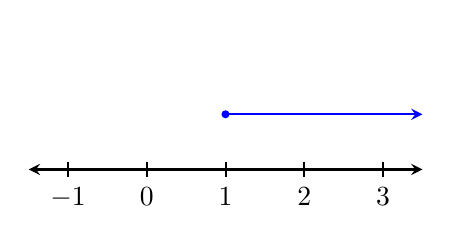
\begin{tikzpicture}
			\draw[stealth-stealth] (-1.5,-.2) -- (3.5,-.2);
			\foreach \X in {-1,...,3}
			{\draw (\X,-0.1) -- (\X,-0.3) node[below]{$\X$}; 
			}

%		   \pic{plot inequality={0.05*(\x*\x-1)>sin(deg(\x*3)) }{-3.5}{3.5}{0}}; \node at (5.5,0) {\(\frac{(x^2-1)}{20}>\sin(3x)\)};
%		   \pic{plot inequality={0.05*(\x*\x-1)<sin(deg(\x*3)) }{-3.5}{3.5}{1}}; \node at (5.5,1) {\(\frac{(x^2-1)}{20}<\sin(3x)\)};
		   \pic{plot inequality={\x>1}{0}{3.5}{0.5}};
		\end{tikzpicture}
		\item $x\leq1$:\\
		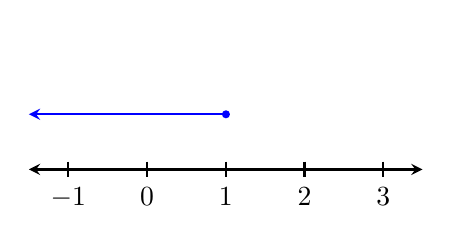
\begin{tikzpicture}
			\draw[stealth-stealth] (-1.5,-.2) -- (3.5,-.2);
			\foreach \X in {-1,...,3}
			{\draw (\X,-0.1) -- (\X,-0.3) node[below]{$\X$}; 
			}
		 
		   \pic{plot inequality={\x<1}{-1.5}{1.5}{0.5}};
		\end{tikzpicture}
	\end{enumerate}		
\end{enumerate}
}
\begin{question}{判別不等式之解}{example}
	\begin{enumerate}
		\item 下列哪些值是不等式 $3x-5>3$ 的解?\\[8pt]
			\twoch{$1$}{$2$}{$3$}{$4$}
		\item $x=3$ 可以是下列哪些不等式的解?\\[8pt]
			\twoch{$2x-1>4$}{$3x+6\geq20$}{$\cfrac{3x}2+1\leq5$}{$-2x+3<1$}
		\item 在數線上圖示下列不等式:
		\begin{enumerate}[label=(\arabic*)]
			\item $x<-1$
			\item $x\geq2$
		\end{enumerate}			
	\end{enumerate}	
\end{question}
\vspace{35ex}
\begin{observing}
	\begin{enumerate}
		\item $x=-3$ 可以是下列哪些不等式的解?\\[8pt]
			\twoch{$-5x-9<4$}{$2x+6>0$}{$\cfrac{x}3+1<2$}{$2x<1$}
		\item 在數線上圖示下列不等式:
		\begin{enumerate}[label=(\arabic*)]
			\item $x\geq3$
			\item $x<-2$
		\end{enumerate}			
	\end{enumerate}
\end{observing}


\subsection{直線方程式的應用}

\subsection{圓與直線的關係}

\end{document} 




